\chapter[Case Studies]{Case Studies:
  Foundations of Computer Science Exercises 4 and 6, and
  Prolog Technology Theorem Prover}
\label{case}

This chapter provides an analysis of the use of PrologPF in
expressing algorithms typical of higher-order functional programming, and
testing the use of PrologPF on a substantial problem.
The sample programs have been taken from the functional programming
exercises in Standard ML \cite{MTH90} 
set to undergraduate students on a university Computer
Science class \cite{Pau88}, and the
Prolog Technology Theorem Prover from SRI \cite{Sti88}.

The first example, Exercise 4, introduces the style of
functional programming in PrologPF
and shows the use of a Prolog relation within
a function definition.  The second example, Exercise 6, uses higher-order
functional programming to create infinite lists, and shows how this
style of functionally implemented data structure can be used within
a relational program.  The Prolog Technology Theorem Prover, with a
large test problem, provides a suitabel body of Prolog code for transferral
to PrologPF, for potential parallel speedup.

%%%%%%%%%%%%%%%%%%%%%%%%%%%%%%%%%%%%%%%%%%%%%%%%%%%%%%%%%%%%%%%
\section{Foundations of Computer Science Exercise 4 - Routes} %
%%%%%%%%%%%%%%%%%%%%%%%%%%%%%%%%%%%%%%%%%%%%%%%%%%%%%%%%%%%%%%%

\subsection{Problem Description}
%%%%%%%%%%%%

The sample problem is to form the transitive closure of a relation.  A function
\texttt{routes} is to be defined which, given a list representing the arcs of an
acyclic graph, returns a similar list representing all possible connections.
The initial list representing the graph can be [(a,b),(b,c),(b,d),(d,e)], for
the graph given in Figure \ref{ex4_1}.

\begin{figure}[htbp]
\vspace{5mm} \hbox to \hsize{\hfill \psfig{file={case/ps/ex4_1.ps}} \hfill}
\caption{Initial acyclic directed graph for Exercise 4.}
\vspace{5mm}
\label{ex4_1}
\end{figure}

The function call \texttt{routes([(a,b),(b,c),(b,d),(d,e)])} should return the
expanded list
\texttt{[(a,c),(a,d),(a,e),(b,e),(a,b),(b,c),(b,d),(d,e)]}, representing the
graph in Figure \ref{ex4_2}.

\begin{figure}[htbp]
\vspace{5mm} \hbox to \hsize{\hfill \psfig{file={case/ps/ex4_2.ps}} \hfill}
\caption{Complete graph for Exercise 4.}
\vspace{5mm}
\label{ex4_2}
\end{figure}

\subsection{Startpoints and Endpoints}
%%%%%%%%%%%%

The final algorithm will use some utility functions to produce intermedate results.
Firstly, we define the function \texttt{startpoints} which, given a list
of arcs and a node, will return the sublist of arcs with that node as the endpoint.
\begin{verbatim}
fun startpoints([],Z)            = [];
    startpoints([(X,Z)|Pairs],Z) = [X|startpoints(Pairs,Z)];
    startpoints([(X,Y)|Pairs],Z) = startpoints(Pairs,Z).
\end{verbatim}
The functional syntax of PrologPF is clearly similar to Standard ML \cite{MTH90}.  The
eager evaluation semantics are also similar, but PrologPF is typeless.  The Prolog syntax
for variables and lists has been preserved.
The function definition is terminated with a full stop (.), allowing
the definition to be a readable term in standard Prolog \cite{DEDC96}.  The functional
support in PrologPF can be added to a Prolog compiler without change to the parser.
A PrologPF program without functions has the same syntax as an identical
Prolog program.  The PrologPF definition of \texttt{startpoints} has exploited the
use of a logical variable \texttt{Z} in the second case. The definition assumes an
ordering of the cases, with the first left-hand-side to successfully unify with the 
arguments in the call being
deterministically selected for the next reduction step.  The function could be written
with an \textit{if-then-else} expression replacing the second and third cases, avoiding
the use of logical variables, in which case the code would be almost identical to the
same function written in ML. 

To produce a sublist of endpoints from a given startpoint, a similar function 
\texttt{endpoints} is needed:
\begin{verbatim}
fun endpoints([],X)            = [];
    endpoints([(X,Y)|Pairs],X) = [Y|endpoints(Pairs,X)];
    endpoints([(Z,Y)|Pairs],X) = endpoints(Pairs,X).
\end{verbatim}

\subsection{Allpairs and append}
%%%%%%%%%%%%

Here we develop the function \texttt{allpairs} which produces the 
cartesian product of two lists of pairs.  The function will use a
utility function \texttt{append}, which returns the list formed from
appending its two actual arguments:
\begin{verbatim}
fun append(X,Y) = if append(X,Y,Z) then Z.
\end{verbatim}
The PrologPF \textit{if-then-else} expression has a relational goal as
the condition.  If the goal succeeds (with an associated unifier) then
the result is the \textit{then}
expression, otherwise it is the \textit{else} expression.  The \textit{if-then}
form used in the example has an implicit \textit{else} expression of \texttt{fail}.
The example of \texttt{append} shows the straightforward mapping of a particular mode
of a relation into an equivalent function.  PrologPF distinguishes between functions
and relations of the same name if they have differing numbers of arguments.  Curried
use of the PrologPF function \texttt{append} is permitted, where the function call will
have fewer than two actual arguments.  In the simplest definitions, such as \texttt{append},
the equivalent relation will often have one \textit{more} argument than the equivalent
function.  This enables PrologPF to provide a set of library functions representing many
of the relations expected in a standard Prolog library, using the same names.

The first stage to provide the cartesian product of two lists is to define a function
which pairs one element with every value of a list, producing a list of pairs.  This
function, \texttt{pairx} is defined as follows:
\begin{verbatim}
fun pairx(_,[])     = [];
    pairx(X,[Y|Ys]) = [(X,Y)|pairx(X,Ys)].
\end{verbatim}
The function \texttt{pairx} illustrates the use of ``\texttt{\_{}}'' to
represent an anonymous variable, consistent with the syntax in both Prolog and ML.

The function \texttt{allpairs} also uses an anonymous variable, and the functions
\texttt{append} and \texttt{pairx}:
\begin{verbatim}
fun allpairs([],_)      = [];
    allpairs([X|Xs],Ys) = append(pairx(X,Ys), allpairs(Xs,Ys)).
\end{verbatim}

In common with the global definition of relational procedures, 
PrologPF has no support for the lexical scoping of function definitions.
The equivalent functions in ML could be nested to place the value of \texttt{x}
in \texttt{allpairs} within the scope of \texttt{pairx}:
\begin{verbatim}
fun allpairs([],_)       = [];
    allpairs((x::xs),pairs) = 
        let
           fun pairx([])    = [];
               pairx(y::ys) = (x,y)::pairx(ys).
        in
           pairx(pairs) @ allpairs(xs,pairs)
        end;
\end{verbatim}
The ML definition also takes advantage of the infix definition of the ML library
append function \texttt{@}.

\subsection{Addnew}
%%%%%%%%%%%%

We can call a list of arcs \textit{complete} if whenever it contains two arcs
\texttt{(a,b)} and \texttt{(b,c)} then it also contains the arc \texttt{(a,c)}.
The function \texttt{addnew}, given an arc and a complete list of arcs, will return
a complete list including the new arc.  For example, \texttt{addnew((a,b),[(b,c)])}
will return \texttt{[(a,b),(b,c),(a,c)]}.
Functions \texttt{addall} and \texttt{addnew} are mutually recursive.  Firstly,
the function \texttt{addall} uses \texttt{addnew} to insert each arc in its first
argument into the complete list given as its second.
\begin{verbatim}
fun addall([],Pairs)      = Pairs;
    addall([P|Ps], Pairs) = addall(Ps, addnew(P,Pairs)).
\end{verbatim}
The function \texttt{addnew}
has an arc as its first argument and a complete list of arcs as its second.
\begin{verbatim}
fun addnew(Pair,[])      = [Pair];
    addnew((X,Y), Pairs) =
        if (member((X,Y),Pairs); X=Y)
        then Pairs
        else addall( append( allpairs( startpoints(Pairs,X), [Y]),
                             allpairs( [X], endpoints(Y,Pairs))),
                     [(X,Y)|Pairs]).
\end{verbatim}
In the general case, \texttt{addnew} will prepend the new arc \texttt{(X,Y)} onto the complete
list of arcs given as a second argument, and will call \texttt{addall} to
recursively add all the arcs leading to \texttt{X} or leading from \texttt{Y}.  The
example \textit{if-then-else} expression in \texttt{addnew} further illustrates the
use of a relational goal as the condition, in which the disjuctive operator \texttt{;} is
used to represent \texttt{or\_{}else}.  The operator has the same left-to-right interpretation
as in sequential Prolog.

\subsection{Routes}
%%%%%%%%%%%%

Finally the function \texttt{routes}, given an arbitrary list of arcs as its argument,
will recursively call \texttt{addnew} to add each arc to an accumulated complete
list:
\begin{verbatim}
fun routes([])            = [];
    routes([(X,Y)|Pairs]) = addnew((X,Y),routes(Pairs)).
\end{verbatim}

The function \texttt{routes} can be exercised by its use in a top level goal such as:
\begin{verbatim}
:- Z = routes([(a,b),(b,c),(b,d),(d,e)])
\end{verbatim}
The goal will succeed with the single solution,\\
\centerline{\texttt{Z = [(a,c),(a,d),(a,e),(b,e),(a,b),(b,c),(b,d),(d,e)]}}

%%%%%%%%%%%%%%%%%%%%%%%%%%%%%%%%%%%%%%%%%%%%%%%%%%%%%%%%%%%%%%%
\section{Foundations of Computer Science Exercise 6 - Primes} %
%%%%%%%%%%%%%%%%%%%%%%%%%%%%%%%%%%%%%%%%%%%%%%%%%%%%%%%%%%%%%%%

This exercise exploits the higher-order programming capabilities of PrologPF to
simulate lazy execution for the definition of infinite lists.  A function
\texttt{primes} is defined using a sieve algorithm to return
an infinite list of primes.  This
function is used in the simple definition of a relation \texttt{prime(P)} which
succeeds for prime \texttt{P}, and can be used as a generator for primes within
a relational goal.

\subsection{Infinite lists}
%%%%%%%%%%%%

A carefully designed PrologPF term can be used to represent an infinite list.  The
term can be a compound term \texttt{item(X,Xf)} where \texttt{X} is the value to be 
found at the
head of the list, and \texttt{Xf} is a \textit{function} which can be called to
return the tail of the list.  The tail of the infinite list will itself be a compound
term of the same structure.

Thus, for example, the infinite list of the natural numbers can
be represented by the PrologPF term:\\
\centerline{\texttt{item(1, lambda([],item(2,lambda([],item(3,...))))) }}
This term can be constructed by the function \texttt{makeints}:
\begin{verbatim}
fun makeints(N) = item(N, lambda([], makeints(N+1))).
\end{verbatim}

\subsection{Head, tail and nth}
%%%%%%%%%%%%

As with the usual Prolog-style lists, functions such as \texttt{head} and
\texttt{tail} can be created which extract the
components of the infinite lists:
\begin{verbatim}
fun head(item(I,_)) = I.

fun tail(item(_,Xf)) = Xf @ [].
\end{verbatim}
The \texttt{tail} function uses the explicit application operator \texttt{@} to
evaluate the function representing the tail of the list.  With the example
of the term representing the infinite list of integers given above, \texttt{tail}
will evaluate \texttt{lambda([],item(2,lambda(..))) @ []}, returning the term
\texttt{item(2,lambda(..))}.

An additional utility function common in the use of lists is \texttt{nth}, returning
the $n^{th}$ element of a list:
\begin{verbatim}
fun nth(S,1) = head(S);
    nth(S,N) = nth(tail(S),N-1).
\end{verbatim}
The definition of \texttt{nth} illustrates the use of \texttt{head} and \texttt{tail}
to abstract the definition of the term used to represent the infinite list.  The
function \texttt{nth} can be used in a curried form, where \texttt{nth(S)} represents
a function which when applied to an integer will return the element of the list \texttt{S}
indexed by that integer.

\subsection{Filters}
%%%%%%%%%%%%

The sieve algorithm used to produce the infinite list of primes requires a 
higher-order function
\texttt{filters} which, given a selection function and an infinite list, returns
the list containing those elements for which the selection function is true.

An example of a selection function, and that used in \texttt{primes}, is
\texttt{notdiv}, returning \texttt{true} if the first argument is not an exact
divisor of the second:
\begin{verbatim}
fun notdiv(X,Y) = if (Y mod X =\= 0) then true else false.
\end{verbatim}
The function uses the Prolog library relation \texttt{=$\backslash$=} and the
Prolog arithmetic function \texttt{mod}, as an alternative to defining these as
PrologPF functions for a simpler boolean definition of \texttt{notdiv}.

The function \texttt{filters} applies the selection function given as the first 
argument in the condition of an \textit{if-then-else} expression.  The condition is
interpreted as a relational goal, and \texttt{filters} exploits the
PrologPF treatment of the function call \texttt{F @ [X]} in this position as the goal
\texttt{(F @ [X]) = true}.
\begin{verbatim}
fun filters(F, item(X,Xf)) =
        if (F @ [X])
        then item(X,lambda([], filters(F, Xf @ [])))
        else filters(F, Xf @ []).
\end{verbatim}
The function illustrates the use of higher-order variables to represent functions,
the explicit application of those functions using the operator \texttt{@}, and
the creation of nameless functions using \texttt{lambda}.

\subsection{Primes}
%%%%%%%%%%%%

Given the definition of the term used to represent an infinite list, and the
utility functions defined above, the definition of the function \texttt{primes}
is straightforward:
\begin{verbatim}
fun primes(item(X,Xf)) =
        item(X, lambda([], primes(filters(notdiv(X), Xf @ [])))).
\end{verbatim}
Given an infinite list of integers starting with a prime, the function will return
the infinite list beginning with that number, followed by the infinite list of
the application of \texttt{primes} to the list having filtered out all the elements
divisible by the first prime.  The encapsulation of the tail of the list within
the \texttt{lambda} expression serves to delay the evaluation of the tail, avoiding
an infinite loop.

The functional definition and creation of infinite lists in PrologPF has a natural 
use within relations.  Firstly, a relation \texttt{next\_{}prime} can be defined
which succeeds for each element in a list:
\begin{verbatim}
next_prime(Primes,P) :- P = head(Primes).
next_prime(Primes,P) :- next_prime(tail(Primes),P).
\end{verbatim}
Finally, the relation \texttt{prime(P)} can be defined which succeeds for each prime
integer \texttt{P}, and provides a generator for the primes:
\begin{verbatim}
prime(P) :- next_prime(primes(makeints(2)), P).
\end{verbatim}
A top level goal \texttt{:- prime(P)} provides an infinite sequence of solutions
\texttt{P=2, P=3, P=5,\ldots}.

%%%%%%%%%%%%%%%%%%%%%%%%%%%%%%%%%%%%%%%%%%%%
\section{Prolog Technology Theorem Prover} %
%%%%%%%%%%%%%%%%%%%%%%%%%%%%%%%%%%%%%%%%%%%%
\label{case_pttp}

The Prolog Technology Theorem Prover (PTTP) developed by Mark Stickel \cite{Sti88}
improves upon the incomplete semantics of Prolog by:
\begin{enumerate}
\item{Using a sound unification algorithm with an occurs check.}
\item{Permitting general logical formulas to be used in clauses, rather than just the
Horn clauses accepted by Prolog.}
\item{Replacing the unsound depth-first search with an iterative deepening search.}
\end{enumerate}
PTTP also retains information on which formulas where used for each inference so that
the proof can be printed.  The theorem prover tranforms the assigned problem into a
suitable Prolog program, which is then compiled and executed using a standard Prolog
compiler.  PTTP is approximately 1500 lines of Prolog code, including comments,
divided into the following parts:
\begin{enumerate}
\item{The code to transform the general assigned problem into a suitable Prolog
program.}
\item{The utility relations used by that program to ensure its sound execution, for
  example the unification algorithm and various list utility predicates.}
\item{The clauses representing the sample problems.}
\end{enumerate}
The sample problems used in the case study result in Prolog programs of 400 to 500
lines of Prolog code, including the needed utilities.

\subsection{Chang and Lee example 2}
%%%%%%%%%%%%

As an example of the execution of the Prolog Technology Theorem Prover, 
the first sample problem is taken from \cite{CL73}:
\begin{verbatim}
p(e,X,X).
p(X,e,X).
p(X,X,e).
p(a,b,c).
p(U,Z,W) :- p(X,Y,U), p(Y,Z,V), p(X,V,W).
p(X,V,W) :- p(X,Y,U), p(Y,Z,V), p(U,Z,W).
query :- p(k(X),X,k(X)).
\end{verbatim}
A Prolog term representing this problem is transformed into a Prolog program which
is run producing the following proof:
\begin{verbatim}
Goal#  Wff#  Wff Instance
-----  ----  ------------
  [0]    7   query :- [1].
  [1]    5      p(b,a,c) :- [2] , [9] , [10].
  [2]    6         p(c,a,b) :- [3] , [4] , [8].
  [3]    3            p(c,c,e).
  [4]    5            p(c,b,a) :- [5] , [6] , [7].
  [5]    4               p(a,b,c).
  [6]    3               p(b,b,e).
  [7]    2               p(a,e,a).
  [8]    1            p(e,b,b).
  [9]    3         p(a,a,e).
 [10]    2         p(c,e,c).
\end{verbatim}
The Prolog program representing the transformed problem contains a small number of
relations using \textit{cut}, which can be replaced with PrologPF functions.  For
example, the relation \texttt{identical\_{}member} can be replaced with a function:
\begin{verbatim}
identical_member(X,[Y|_])  :-
      X == Y,
      !.                        % note presence of cut
identical_member(X,[_|L]) :-
      identical_member(X,L).
\end{verbatim}
The equivalent function in PrologPF which avoids the use of \textit{cut} is as
follows: 
\begin{verbatim}
fun identical_member(X,[]) = false;
    identical_member(X,[Y|L]) =
        if (X == Y)
        then true
        else identical_member(X,L).
\end{verbatim}
The compiled PrologPF version of the Chang Lee example completes on a single cpu with
the PrologPF partitioning depth limit set to 1 (i.e.\ a single partition) in
2187 milliseconds.  The execution on the distributed PrologPF system with a
suitable depth limit $L=23$ for parallel execution produces the
runtimes of the graph in Figure \ref{changlee2_L_23_runtime}.

\begin{figure}[htbp]
\vspace{5mm} \hbox to \hsize{\hfill \psfig{file={case/ps/changlee2_L_23_runtime.ps}} \hfill}
\caption{Runtimes for Chang Lee example 2 for $G=1\ldots 30$ and $L=23$.}
\vspace{5mm}
\label{changlee2_L_23_runtime}
\end{figure}

The problem is sufficiently small to limit the runtime to a minimum of about 500
milliseconds.  Another example, provided by Overbeek \cite{DLO87}, provides a much
greater search space and potential for much improved parallel speedup when compiled
with PrologPF.

\subsection{Overbeek example 4}
%%%%%%%%%%%%

An example problem provided by Overbeek \cite{DLO87} has a single cpu runtime on the
processors used by the distributed PrologPF system of over five hours:
\begin{verbatim}
p(e(X,e(e(Y,e(Z,X)),e(Z,Y)))).
p(Y) :- p(e(X,Y)), p(X).
query :- p(e(e(e(a,e(b,c)),c),e(b,a))).
\end{verbatim}
Compilation and execution proceeds in the same manner as for the Chang and Lee
example.

The graph given in Figure \ref{pttp_overbeek_L_130_runtime} shows the improvement in
runtime as processors are added to the group used to execute the problem.

\begin{figure}[htbp]
\vspace{5mm} \hbox to \hsize{\hfill \psfig{file={case/ps/pttp_overbeek_L_130_runtime.ps}} \hfill}
\caption{Runtimes for Overbeek example 4 for $G=1\ldots 42$ and $L=130$.}
\vspace{5mm}
\label{pttp_overbeek_L_130_runtime}
\end{figure}

The improvement is clarified with the speedup graph in
Figure \ref{pttp_overbeek_L_130_spdup} which plots the speedup ratio against the
single cpu case for groups of path processors up to a maximum group size of 42.

\begin{figure}[htbp]
\vspace{5mm} \hbox to \hsize{\hfill \psfig{file={case/ps/pttp_overbeek_L_130_spdup.ps}} \hfill}
\caption{Speedup for Overbeek example 4 for $G=1\ldots 42$ and $L=130$.}
\vspace{5mm}
\label{pttp_overbeek_L_130_spdup}
\end{figure}

The speedup graph shows linear speedup throughout the range of group sizes available.
For some values of $G$, such as 18 and 27, the speedup is greater than the increase in
the number of path processors.  This phenomenon is a result of the single-solution
requirements of the code produced by PTTP.  In a sequential execution, the first
solution found will be that furthest to the left in the depth-first, left-to-right
search tree.  Also, the search tree to the left of that solution will be fully
search before the solution is discovered.  In the distributed execution of PrologPF,
the search tree is partitioned between the available path processors and the first
solution found will be that furthest to the left \textit{within the subtree assigned to
that path processor}.  The paritioning may result in a solution appearing very early
in the subtree assigned to one of the path processors, such that it is found very
quickly.  The situation is illustrated in the simplified diagram in Figure \ref{super_linear}.

\begin{figure}[htbp]
\vspace{5mm} \hbox to \hsize{\hfill \psfig{file={case/ps/super_linear.ps}} \hfill}
\caption{Greater than linear speedup for single-solution problems.}
\vspace{5mm}
\label{super_linear}
\end{figure}

In the single-cpu case, the subtrees labelled A and B in the figure will be searched, taking
at least 520ms, and then the solution \texttt{X} 
will be discovered after at least 2ms in the subtree labelled C.
If the problem is divided between three path processors, then the third path processor will
discover the solution \texttt{X} 
after the partitioning time (20ms) followed by the search to
the solution in subtree B, taking approximately 52ms.  In this simple example, the
shallow positioning of the solution in subtree C gives a speedup for the single-solution
case of approximately 10 with only 3 path processors.  Note that for the all-solutions case,
the subtrees A,B,C,D and E, would all have to be fully searched such that the benefit of
one or more shallow solutions will not be obtained.
The one-solutions requirements of the Prolog Technology Theorem Prover means that with
fortuitous partitioning greater than linear speedup can be obtained.

%%%%%%%%%%%%%%%%%%%%%%%
\section{Conclusions} %
%%%%%%%%%%%%%%%%%%%%%%%

PrologPF provides support for functional programming comparable to that of a typeless ML,
in which some programs have a more convenient expression than their Prolog equivalents.  The
deterministic reduction of functional expressions permits the expression of many algorithms
that would otherwise suggest the use of \textit{cut} in Prolog.

The syntax for functional definition and evaluation in PrologPF is consistent with the
standard Prolog syntax for the relational procedures, such that functions and relations
can be mixed in a program without conflict of programming styles.  Data structures, such
as lists and compound terms, are common to the relational and functional components of
PrologPF.

The combined functional and logic support in PrologPF, with the relational procedures
compatible with standard Prolog \cite{DEDC96}, allow a straightforward conversion of
substantial Prolog programs to equivalent PrologPF programs suitable for execution on
the Delphi Machine.  In the case of the largest program tested, the Prolog Technology
Theorem Prover, a speedup of 40 times using 42 processors was achieved.

%%%%%%%%%%%%%%%%%%%
\section{Summary} %
%%%%%%%%%%%%%%%%%%%

The problem of finding the transitive closure of a relation provides a suitable
exercise for functional programming, with the relation defined as a set of arcs beween
nodes of a graph.  Prolog terms can be used to represent the arcs (i.e.\ the tuple
\texttt{(a,b)} to represent the arc $a\rightarrow b$), and the set of arcs stored in
a Prolog list.  The functions necessary to transform this list into a complete list
representing the transitive closure can be implemented in PrologPF in as straightforward
a manner as in Standard ML \cite{MTH90}.  Functions and terms are typeless in PrologPF,
consistent with the typeless environment of Prolog.  Potential benefits of a polymorphic
type inferencing system as found in ML have not been provided in PrologPF.

The higher-order programming capabilities of PrologPF include the definition of nameless
functions using \texttt{lambda} expressions, and the ability to pass functions as arguments
and return them as results.  These capabilities can be demonstrated in the use
of lazy evaluation in the implementation of infinite lists.  The terms used to represent
the lists contain lambda expressions, and higher-order functions \texttt{head} and
\texttt{tail} are used to extract the elements of the list.  A function \texttt{primes}
can be written to return the infinite list of primes.  The example given shows the
integration of the functional support with a relation \texttt{prime(P)} which succeeds for
any prime, P.  The relation can be used with \texttt{P} an integer, or a 
\texttt{P} a variable which
will be instantiated with a sequence of primes.

The Prolog Technology Theorem Prover is a Prolog program which can transform the predicate
calculus representation of a logic program into an equivalent Prolog program avoiding
some incomplete aspects of Prolog's execution.  Depth-first search is replaced with
breadth-first, and an explicit occurs check is embedded in the code.  The procedures in the
program containing \textit{cut} can be replaced with equivalent functions, and the
resulting program compiled with the PrologPF compiler for a speedup in execution of up
to 40 times on the Cambridge laboratory's 42 workstations.
